% !TeX root = 00main.tex

%%%%%%%%%%%%%%%%%%%%%%%%%%%%%%%%%%%%%%%%%%%%%%%%%%%%%%%%%%%%%%%%%%%%%%%%%%%
% System design
%%%%%%%%%%%%%%%%%%%%%%%%%%%%%%%%%%%%%%%%%%%%%%%%%%%%%%%%%%%%%%%%%%%%%%%%%%%

%%%%%%%%%%
% Overall design  
%%%%%%%%%%

\subsection*{Overall design}

%
% System configuration
%

The design is based on the initial proposal by Matsubara-san, with some modifications to ease installation and improve the coverage of the light on the PMT~array.

\missing[inline]{Furuta-san: picture of LED mounting board}
\missing[inline]{Furuta-san: coordinates of LEDs and associated PMT IDs (if available?)}
\missing[inline]{SJMP: Wavelength spectra for 420~nm and 355~nm LEDs}

\begin{figure}
\begin{center}	
  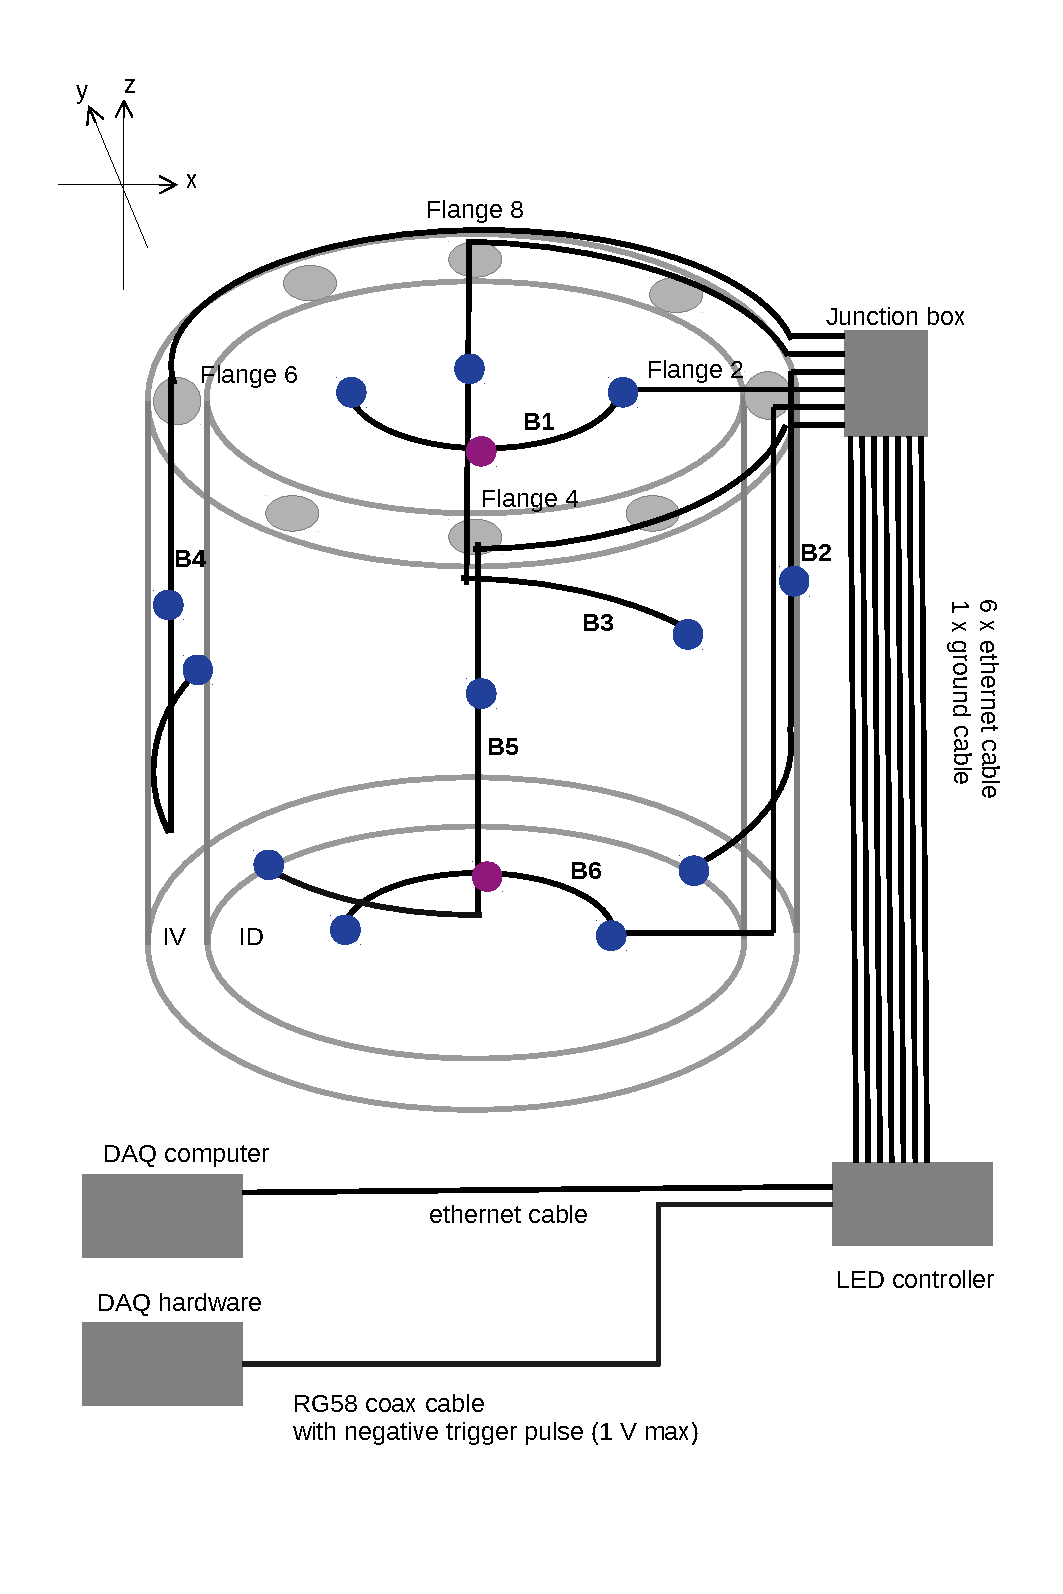
\includegraphics[width=0.75\linewidth]{figures/JSNS2_led_system_overview.pdf}
  \caption{A schematic overview of the nanopulser optical calibration system. The (two) purple points indicate the position of the nanopulser heads (LED driver boards) with a 355~nm LED, the (twelve) blue points indicate nanopulser heads with a 420~nm LED.}
  \label{figure:controlbox}
\end{center}
\end{figure}

\subsubsection*{System configuration}

%
% System configuration
%

\subsubsection*{System performance}

%%%%%%%%%%
% Nanopulser head
%%%%%%%%%%

\subsection*{Nanopulser head}

\begin{figure}
\begin{center}	
  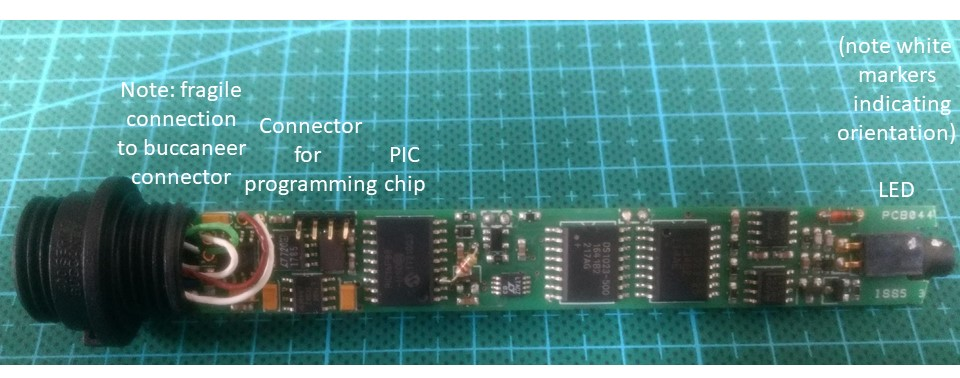
\includegraphics[width=1.0\linewidth]{figures/pulserhead.jpg}
  \caption{Photo of the a nanopulser head, outside of its acrylic housing, with the main components indicated.}
  \label{figure:pulserhead}
\end{center}
\end{figure}

Note that for transfer the maximum energy in a fast pulse, that we found that it is important that the legs of the LEDs are not shortened, but bend out to fit.
\missing[inline]{RW: detailed schematic of the nanopulser head.}

%
% Nanopulser head programming
%

\subsubsection*{Nanopulser head programming}

The nanopulser heads are each programmed for a specific position on the branch and with its own unique ID (1-14). 
The programming can be done separately from the system, as shown in Figure~\ref{figure:pulserhead_programming}, with a custom cable providing the 9~V power for the PIC chip\footnote{Make sure the battery has enough power left to power the PIC chip.}. The code is loaded onto the PIC~chip via a commercial interface (microchip PICkit3) with a custom cable to the nanopulser head. Note that, as shown in Figure~\ref{figure:pulserhead_programming}, the grey lead lines up with the arrow on the PICkit3 interface. On the other side, the green lead is closest to the LED on the nanopulser head. The connector on the nanopulser head is slanted an slightly bend, to make it fit into the nanopulser head's acrylic housing. Therefore, take extra care when connecting to make sure a good contact is make.

The software for the nanopulser head programming can be found on github~\cite{GITHUB_PIC}. This contains a zip file (PICkit3.zip), which contains the windows compatible executable file PICkit3.exe, as well as other (required) input files for the program. It also contains the 14 hex files to be loaded onto the pulser: nanoSlaveTrig\_X.hex, where X is a letter from A-N. This corresponds to pulser ID 1-14, respectively, as shown in Table%~\ref{table:cabling_overview}
 (i.e., A is for pulser head 1, etc.).

The program PICkit3.exe is started by double-clicking (make sure the PICkit3 device is connected and recognised, otherwise the next step is not possible). Next, select the PIC chip to program: under menu `Device family', select {\bf MidRange}. Then, under `Device', select {\bf PIC16F88} (note there are a lot of models). If the set-up is correct, you can now read the PIC chip by pressing the 'Read' button. This take a little and a green progress bar will appear until the commend read has finished. This should change the hex values shown in Program Memory from their default values to all different values. 

If this was successful, load a hex file by clicking `Import Hex' from the `File' menu. Next, click `Write'. Again a green progress bar should appear to show the progress. Wait until the process has been completed. After this, the PIC chip has been programmed and can be disconnected from the power supply and the PICkit3 device.


\begin{figure}
\begin{center}	
  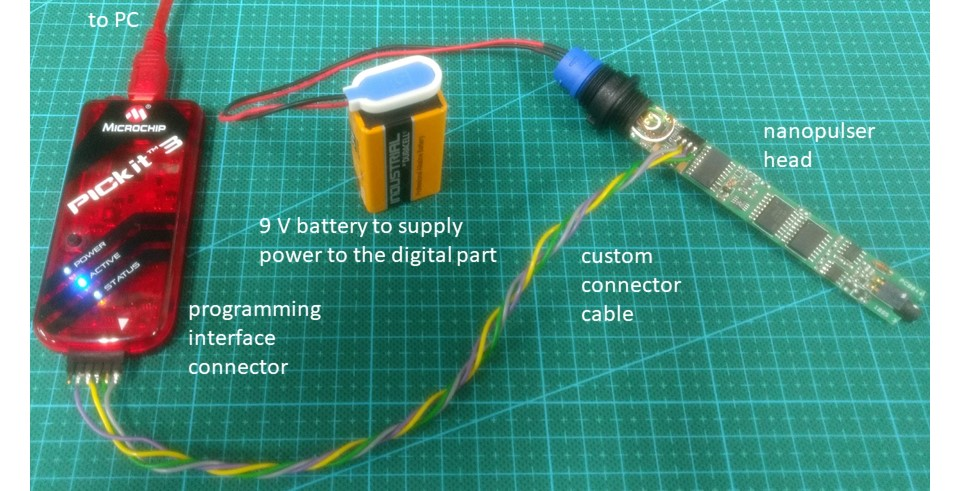
\includegraphics[width=1.0\linewidth]{figures/pulserhead_programming.jpg}
  \caption{The pulser head programming set-up (window10 computer needed, not shown here).}
  \label{figure:pulserhead_programming}
\end{center}
\end{figure}

%%%%%%%%%%
% Nanopulser control box
%%%%%%%%%%

\subsection*{Nanopulser control box}

\begin{figure}
\begin{center}	
  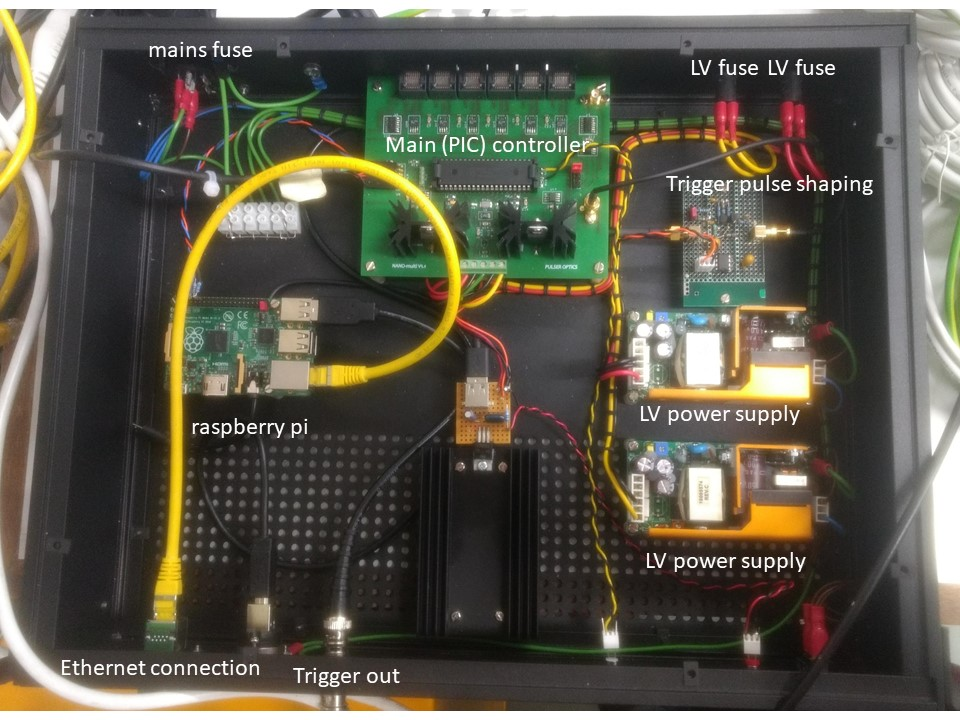
\includegraphics[width=0.75\linewidth]{figures/controlbox.jpg}
  \caption{Photo of the controlbox during commissioning at the University of Sussex, with the main components indicated.}
  \label{figure:controlbox}
\end{center}
\end{figure}
\fix[inline]{RW,SJMP: add details about the voltages (9 V, 7 V, tbc, which is which?)}

One symptom of a blown fuse can be that  the pulser does communicate but either does not produce light, or produces a wide pulse (of the order of 100~ns).

\missing[inline]{RW: details about the delay settings}
\missing[inline]{RW: detailed schematic of the control box}

\subsection*{Cable design}


The ethernet cables should {\bf never} be unplugged from the box, while the power is on, as the power for both the digital electronics, as well as for the pulser circuits runs through them. Accidental hot-swapping can result in one of the fuses blowing. 

\subsubsection*{Junction box}


\begin{figure}
\begin{center}	
  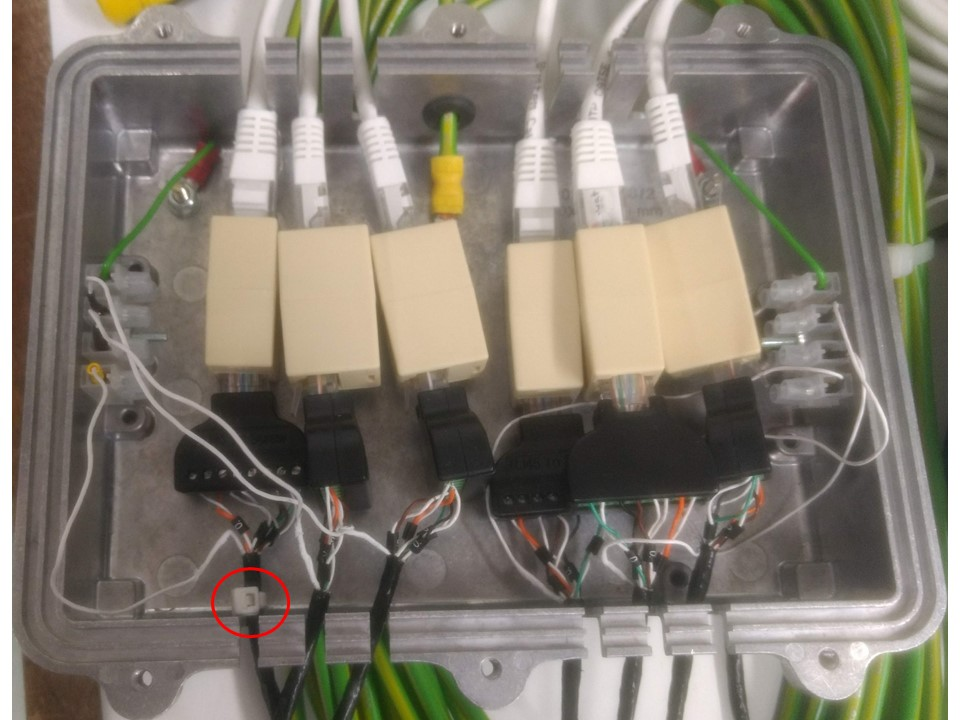
\includegraphics[width=0.75\linewidth]{figures/junction_box.jpg}
  \caption{Photo of the junction during commissioning at the University of Sussex. The ethernet cables on the top connect to the back of the control box (this is labeled 1-6 for the branch numbers). The cables coming from the connector need to be wired to the black eight-way connectors in the pictures (details given below). The cables are then connected with the beige mating connectors. After final assembly in the flange, a tie wrap should be wrapped on each cable as a strain relief. This is demonstrated in the bottom left cable (red circle). }
  \label{figure:junction_box}
\end{center}
\end{figure}



\begin{figure}
\begin{center}	
  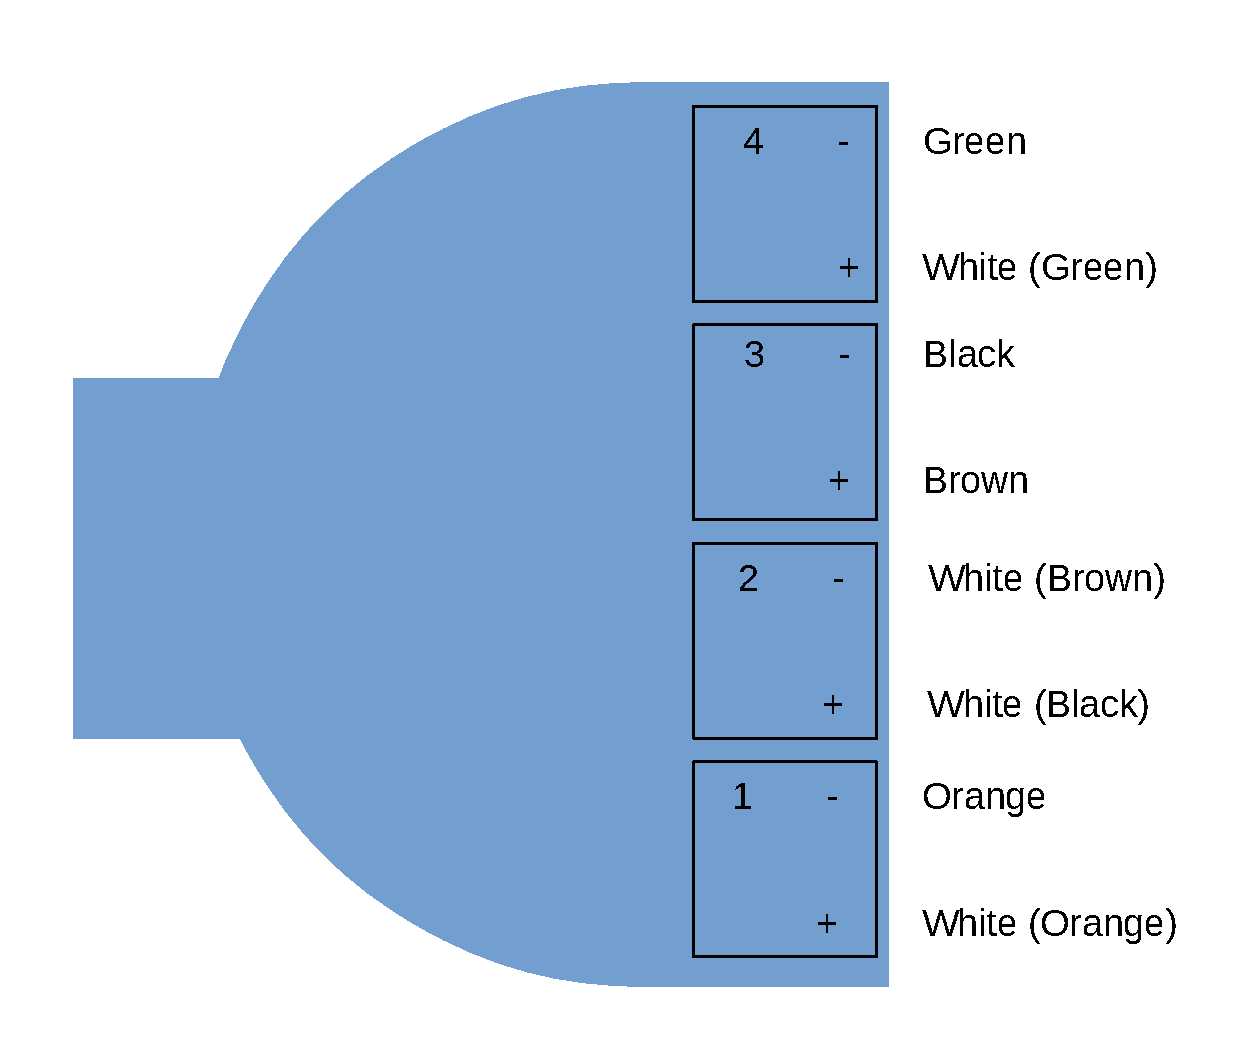
\includegraphics[width=0.5\linewidth]{figures/connector.pdf}
  \caption{A diagram indication how the eight-way connector should be connected to the cables going into the vessel.}
  \label{figure:connector}
\end{center}
\end{figure}

At the final installation, the cables should be wrapped with a tie wrap inside the junction box, to avoid damage to the connection by accidentally pull the cables. Not that the (longer) ground cable also needs to be connected to the junction box chassis (see Figure~\ref{figure:junction_box}).

%%%%%%%%%%
% Nanopulser control  software
%%%%%%%%%%

\subsection*{Control software}

The software is kept in a central github repository\cite{GITHUB_SOFT}.